\documentclass[a4paper, 12pt]{article}
\usepackage[french]{babel}
\usepackage[utf8]{inputenc}
\usepackage[T1]{fontenc}
\usepackage{tikz}
\usepackage{hyperref}
\usepackage{dirtree}

\usepackage[top=2cm,bottom=2cm,left=2cm,right=2cm]{geometry}
\usepackage{graphicx} %'affichage des images
\usepackage{float}

\usepackage{verbatim}

\begin{document}

\title{Conception logiciel \\ Reconnaissance optique de caractère}
\author{GENDARME Steve \and HU Éric \and CHAUVEAU Guillaume}
\maketitle
\begin{figure}[!b]

\includegraphics{img/logo.png}
\end{figure}

\pagebreak

\tableofcontents

\pagebreak
\part{Introduction}
\section{Choix du sujet}
Lors de la première séance, nous avons beaucoup débattu sur le choix du sujet. En effet, Guillaume était intéressé par l'interpréteur de programmes chimiques, Steve plutôt par le Manic Shooter et Éric hésitait entre la programmation chimique et l'OCR.

Nous avons finalement choisi l'OCR, qui semblait être un juste milieu de difficulté, le concept de programmation chimique étant difficile à appréhender et le Manic Shooter est au contraire un grand classique largement choisi par les autres groupes.

\section{Principe d'un OCR}
Un OCR est un logiciel qui va analyser une image pour y trouver du texte et le sauvegarder sous forme numérique. Il se base principalement sur des algorithmes de segmentation d'image pour détecter des zones de texte, des lignes, puis extraire les caractères ou les mots. Ces derniers sont ensuite analysés séparément pour déterminer leur équivalent numérique. La structure du texte peut ensuite être reconstituée pour former le résultat final.

\section{Ce qui existe déjà}
Tesseract est un OCR Open Source que nous avions utilisé au premier semestre en culture numérique. Il a d'abord été développé par HP puis encore aujourd'hui par Google. La version 3 se base sur une segmentation par ligne et par mot puis une reconnaissance mot par mot. \footnote{\href{https://github.com/tesseract-ocr/docs/blob/master/tesseracticdar2007.pdf}{An Overview of the Tesseract OCR Engine}}

L'administration publique utilise aussi un OCR pour scanner des formulaires (création de carte nationale d'identité, passeport...). Toutefois le document à analyser est formaté de manière à favoriser ça lecture: Les caractères sont placés dans des cases (leur position est donc connue) et sont écrits en majuscule (réduction du nombre de cas par caractère).

\pagebreak
\part{Recherches et prototypage}
Pour notre OCR, nous avons choisi une approche de reconnaissance par caractère, plus facile à mettre en œuvre que celle par mot. Le déroulement du programme serait alors constitué de la segmentation de l'image pour séparer les caractères puis la classification de ces caractères. Les informations seraient ensuite ré-assemblées selon la position des caractères.

\section{Classification des caractères}

\subsection{Apprentissage machine}
L'apprentissage machine est une technique d'analyse des données qui permet d'établir un modèle d'une situation à partir de nombreux exemples (provenant d'un ensemble de données, le dataset). Dans notre cas, les exemples sont des images de caractère accompagnées de leur correspondance numérique (le code ASCII du caractère). Le code correspondant à l'image est appelé étiquette (ou label). Le modèle établie nous permet ensuite de faire correspondre une nouvelle image avec une étiquette: c'est la classification.

\subsubsection{Réseaux neuronaux}
Guillaume c'était déjà intéressé à l'apprentissage machine avec \href{https://codelabs.developers.google.com/codelabs/tensorflow-for-poets/}{TensorFlow for poets}, un cours en ligne qui propose d'utiliser un classificateur d'image pour reconnaître des fleurs avec \href{https://www.tensorflow.org/}{TensorFlow}. TensorFlow est une bibliothèque qui offre aux développeurs des outils pour utiliser l'apprentissage machine, notamment pour le traitement d'image. Elle utilise des réseaux neuronaux, une technique d'apprentissage machine. L'utilisation de cet outil était l'une de nos possibilités pour atteindre notre objectif.

Nous nous sommes aussi intéressés à \href{http://dlib.net}{Dlib} qui est une bibliothèque C et Python permettant de faire de l'apprentissage machine et du traitement d'images. Nous l'avons testé en lui fournissant un très grand nombre d'images de chiffres et de lettres et avons obtenue de superbes résultats. En effet, après plusieurs minutes d'entraînement, le programme était capable de reconnaître presque à tous les coup des chiffres ou des lettres.

\subsection{Notre approche pixel par pixel}
Nous avons aussi imaginé notre propre approche du problème. Le modèle pixel par pixel consiste à comparer chaque pixel de l'image à reconnaître avec un modèle obtenu par entraînement, afin justement de reconnaître cette image. Il ne s'appuie donc pas directement sur la forme à analyser mais plutôt sur les correspondances entre pixels.

\section{Orientation du projet}
Nous avons pris la décision d'utiliser notre propre modèle. Nous étions conscients que le taux de succès serait bien plus inférieur à cause de sa simplicité, mais tenter notre propre approche nous semblait plus intéressant que d'utiliser un logiciel qui ferait en grande partie tout le travail sans que nous comprenions son fonctionnement précisément.

La classification allant être notre plus gros défi, nous avons d'abord concentré tous nos effort sur ce problème.

\section{Première implémentation}

\subsection{Le modèle}
Le modèle pixel par pixel est représenté dans le code par la classe CharacterClassifier. Il est constitué d'une liste de matrices formée grâce à un entraînement sur un dataset. Chaque matrice (modèle) est appelée par un label qui correspond au caractère qu'elle illustre.

L’entraînement est très simple. On prend la matrice qui correspond à un certain label et on la compare à toutes les images d'entraînement ayant le même label et on la parcourt. Si à une certaine position la matrice de l'image d'entraînement vaut 0, c'est-à-dire qu'elle correspond à un pixel noir, on ajoute 1 à la même position sur la matrice du modèle. Ou sinon, on lui enlève 1. On répète l'opération pour tous les labels.
A la fin de l'entraînement on obtient donc pour chaque caractère, une matrice unique.

Comme dit plus haut, notre prédiction se base sur les correspondances entre pixel. Cela est très facile à implémenter. Il suffit, pour chaque modèle de la base de donnée, de sommer la valeur des points de correspondance avec l'image à prédire. Nous appellerons score, cette somme. Lorsque deux points ne correspondent pas, on soustrait la valeur du point provenant du modèle au score. Ainsi, chaque pixel à une importance. Cependant, cela donne aussi une grande importance au "blanc" dans l'image. Puis nous divisions ce score par la somme de l'ensemble des valeurs du modèle afin d'obtenir un taux pour chaque label. En fin, le label de la matrice dont le score était le plus important était considéré le résultat de la prédiction.

\subsection{Des premiers résultats encourageants}
L'ébauche du Classifier étant finie, il fallu faire des tests. Pour cela, nous avons créé une dizaines d'exemplaires de 3 lettres, 'A', 'B' et 'C'. Nous avons entraîne le modèle et lui avons fait deviner, avec de nouveaux exemplaires, les lettres 'A', 'B', et 'C'. Cela marchait avec une moyenne d'environ 90\% de précision. Les taux de correspondance étaient plutôt hauts pour la lettre correspondante (~0.90)

\subsection{A l'aide, il faut sauver nos données d'entraînement!}
Pour ne pas avoir à recréer les modèles à chaque lancement, nous avons implémenté une sauvegarde.

Nous avions d'abord conçu un programme qui enregistre notre liste de modèles sous forme de fichiers textes. Il fallait alors parcourir ce fichier pour ré-instancier les objets correspondants. Nous nous somme ensuite tournés vers un module de la bibliothèque standard de Python, \href{https://docs.python.org/3.5/library/pickle.html}{pickle}, qui automatise ce processus. L'avantage est qu'en cas de changement de représentation des modèles, le code de sauvegarde reste inchangé. Pickle va aussi ré-instancier tout les objets afin d'obtenir au chargement la même structure qu'à l'enregistrement.

\subsection{Un nouveau dataset}

Les résultats du modèle étant concluants, nous avons décidé de passer à un dataset plus conséquent. Il nous fallait donc un très grand nombre d'images de chiffres et de lettres. Étant donné qu'il aurait était très long de les créer nous-même, nous avons cherché ce qui existait déjà sur internet. Nous avons ainsi trouvé  \href{http://yann.lecun.com/exdb/mnist/}{le dataset MNIST} qui contient 60 000 images de chiffres labellisés.

\begin{figure}[H]
  \centering
  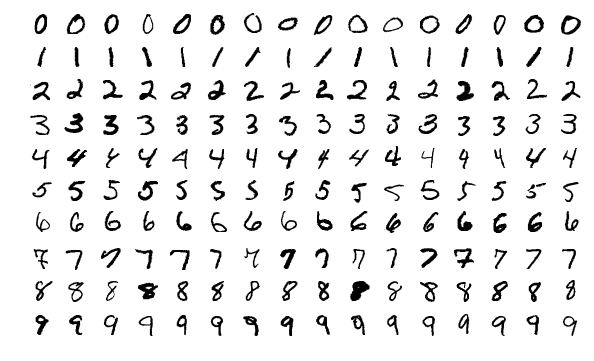
\includegraphics[scale=0.55]{img/mnist.png}
  \caption{Exemple d'image contenu dans le dataset MNIST}
\end{figure}

Ce dataset est séparé en deux fichier binaire que nous allions devoir lire. Le premier contenant les images et le second les labels. Leur structure est :
\begin{itemize}
	\item Pour le fichier contenant les images :
	\begin{itemize}
		\item Un nombre entier sur 32 bit représentant le nombre magique, qui est une constante permettant de désigner le format du fichier. (2049)
		\item Un nombre entier sur 32 bit représentant le nombre d'images. (60 000)
		\item La hauteur en pixel des images. (28)
		\item La largeur en pixel des images. (28)
		\item Puis, chaque octet représentera un pixel.
	\end{itemize}
	\item Pour le fichier contenant les images :
	\begin{itemize}
		\item Un nombre entier sur 32 bit représentant le nombre magique. (2051)
		\item Un nombre entier sur 32 bit représentant le nombre de labels. (60 000)
		\item Puis, chaque octet représentera un label.
	\end{itemize}
\end{itemize}

Nous avons ainsi créé une fonction qui lie chacune de ces informations afin d'en ressortir un dictionnaire dont les clefs sont les labels et les valeurs des listes de PixelMatrix (représentation d'une image).

Le dataset MNIST ne contenant que des chiffres, nous utiliserons  \href{https://www.nist.gov/itl/iad/image-group/emnist-dataset}{la base EMNIST} qui est une version étendue de MNIST contenant en plus des images de chiffres, des images de lettres.

En entraînant notre modèle avec cette dernière, les résultats étaient catastrophiques. En effet, les taux, étaient assez faible (60\% à 70\% seulement) et le poids correspondant au bon label étaient souvent dans le dernier tier.

Pour avoir un aperçu du problème, nous avons pensé à une approche graphique: visualiser les zones de correspondance entre la lettre à deviner et les 3 premières prédictions puis, afin de cerner encore mieux le problème, superposer les 2 lettres en utilisant la classe PixelMatrix ainsi que les librairies numpy et mathplotlib.

Voici un exemple parmi les résultats obtenus:\ref{fig0}
\begin{figure}[!ht]
\centering
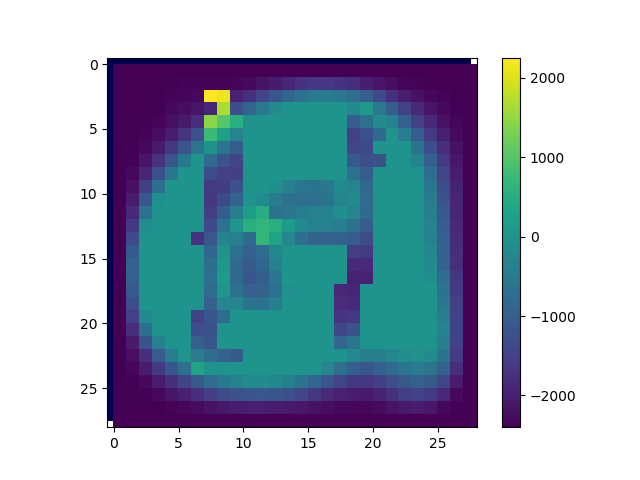
\includegraphics[scale=0.55]{img/pix_corc2.png}
\caption{En bleu-vert, les zones neutres. En jaune, les zones de correspondance entre les 2 matrices. En violet les zones ne correspondant qu'à l'image}
\label{fig0}
\end{figure}

Au final, visualiser les zones de correspondance ne nous a pas tellement aidé à résoudre le problème algorithmique.

\pagebreak
\part{Implémentation finale}
Dans cette partie, nous allons présenter le fonctionnement de notre OCR tel qu'il est à sa première version stable.

\section{Segmentation d'image}
Pour simplifier les opérations de traitement lors de la segmentation mais aussi de la classification, nous commençons par binariser l'image d'entrée. Un pixel noir (allumé) fait donc partie d'un caractère contrairement à un pixel blanc (éteint). Cette opération de seuillage est facile à réaliser car nous partons du principe que l'image contient du texte écrit avec une encre sombre sur du papier blanc. L'image étant en couleur, elle est d'abord passée en niveaux de gris, puis le seuil est automatiquement déterminé avec la moyenne des extremums de l'intensité. Nous imposons aussi des règles d'écriture:
\begin{itemize}
\item Les caractères doivent être séparés (écriture non cursive)
\item Les caractères supportés sont les chiffres de 1 à 9 et les lettres majuscules de A à Z.
\end{itemize}

\begin{figure}[!ht]
\centering
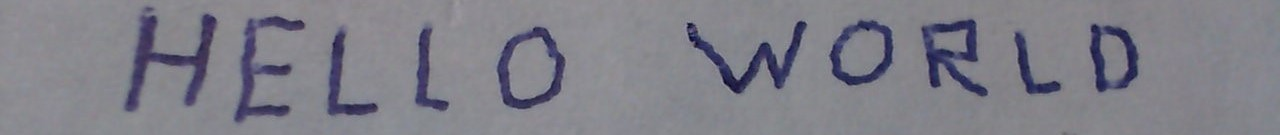
\includegraphics[scale=0.3]{img/text2.jpg}
\caption{Exemple d'image de départ.}
\end{figure}

Nous procédons ensuite à une passe d'érosion qui permet d'augmenter l'épaisseur des caractères. Nous utilisons la bibliothèque \href{https://pypi.python.org/pypi/Pillow}{Pillow} pour manipuler nos images, et celle-ci propose justement un module d'opérations morphologiques. Ce module permet d'écrire ses propres opérations mais vient avec des opérations pré-établies comme "erosion4" qui, pour chaque pixel (i, j) d'une image va modifier sa valeur par le minimum entre chacune des valeur des pixels sur les cotés, au dessus et en dessous. Cette opération rajoute une bordure noire à l'image qui est alors découpée pour l'enlever.

\begin{figure}[!ht]
\centering
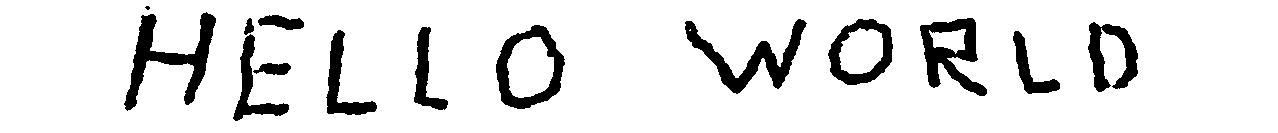
\includegraphics[scale=0.3]{img/text2_bin.jpg}
\caption{L'image après la binarisation et l'érosion.}
\end{figure}

Le choix d'une image binaire impact la précision de notre OCR. En effet, les nuances grises qui bordent les caractères sont soit perdues, soit augmentées, alors que leur valeur nuancée peut avoir un rôle dans la classification.

\subsection{Recherche de forme}
Le sujet nous impose à traiter des images de texte en écriture manuscrite, mais nous avons décidé d'imposer des règles d'écriture pour simplifier le problème. Les caractères devront donc être écrits droit et séparés les uns des autres.

La première étape pour séparer les caractères consiste à rechercher toutes les formes de l'image. Notre image étant binaire, les formes sont donc simplement des ensembles de pixels allumés voisins entre eux.

\begin{figure}[!ht]
\centering
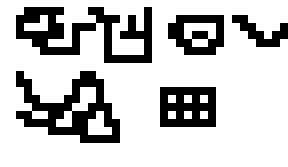
\includegraphics[scale=1]{img/shape.jpg}
\caption{Exemple qui illustrera l'algorithme.}
\end{figure}

L'algorithme commence par parcourir l'image pour y trouver un pixel allumé (appelé un point, les pixels éteints n'en sont pas): c'est le point de départ. Ce point est placé dans une file d'attente de traitement de rangée. Une rangée est une ligne continue de points. Elle peut être verticale ou horizontale, le mode de traitement étant fixé au démarrage.

\begin{figure}[!ht]
\centering
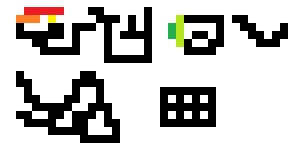
\includegraphics[scale=1]{img/shape_row.jpg}
\caption{Exemples de rangées en mode horizontal (tons rouges) et vertical (tons vert).}
\end{figure}

L'algorithme va ensuite rechercher tous les voisins (donc tous les points d'une rangée) pour chaque point dans la file. L’intérêt de la file va se montrer lorsque d'autres points vont y être ajoutés pendant l'exécution. Dès qu'un nouveau point de la rangée est découvert, il va être effacé de l'image et retiré de la file d'attente s'il y était présent pour éviter qu'il ne soit traité plusieurs fois. Il est ensuite stocké avec les autres points de la forme.

L'étape suivante est de rechercher des points voisins dans les rangées précédentes ou suivantes pour les ajouter à la file (les rangées pouvant être verticale ou horizontale, les termes "précédentes" et "suivantes" sont utilisés pour généraliser "au dessus"/"à gauche" et "en dessous"/"à droite"). Pour cela on vérifie d'abord si ces rangées existent puis, pour éviter de mettre en file d'attente des points de la même rangée, si le point précédemment traité dans la rangée n'a pas déjà été ajouté à la file (une variable stocke cet état séparément entre la rangée précédente et la suivante).
\begin{itemize}
\item Si le point précédent a été mis en file d'attente et que le pixel de la rangée voisine est un point alors on ne fait rien.
\item Si ce n'est pas un point on indique que le point précédent n'a pas été mis en file.
\item Enfin, si c'est un point et que le point précédent n'a pas été mis en file, on y place le point voisin et on note que le point précédent a été mis en file.
\end{itemize}

\begin{figure}[!ht]
\centering
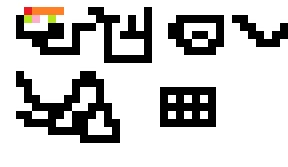
\includegraphics[scale=1]{img/shape_row_neighbors.jpg}
\caption{En rouge le point de départ, en orange les points de la rangée, en vert les points des rangées voisines mis en file d'attente et en rose les points des rangées voisines ignorés.}
\end{figure}

\begin{figure}[!ht]
\centering
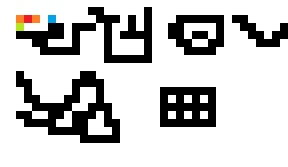
\includegraphics[scale=1]{img/shape_row_neighbors_2.jpg}
\caption{Lors du passage au deuxième point de la file. Les points en bleu sont ceux déjà dans la file.}
\end{figure}

Cette étape est aussi appliquée pour le premier pixel qui n'appartient pas à la rangée, pour traiter les points ayant un coin en contact avec celle-ci.

\begin{figure}[!ht]
\centering
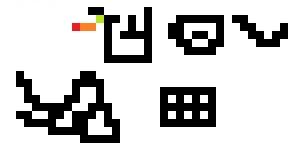
\includegraphics[scale=1]{img/shape_row_neighbors_corner.jpg}
\caption{Ajout des points aux coins de la rangée.}
\end{figure}

\subsection{Reconstitution des caractères et positionnement}
L'algorithme de recherche de forme n'est pas fiable pour extraire un caractère car ce dernier peut être coupé par du bruit et donc être considéré comme deux formes séparées. Il est nécessaire de reconstituer les caractères dans leur entièreté.

\begin{figure}[!ht]
\centering
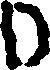
\includegraphics[scale=1]{img/1-9.jpg}
\caption{Exemple d'un "D" composé de deux formes.}
\end{figure}

La recherche des formes s'effectue après la séparation par ligne, on en déduit que les formes au-dessus les unes des autres font partie du même caractère. Il faut projeter les formes sur l'axe horizontal pour repérer l'endroit où les groupes de formes sont séparés par un espace. Pour cela, l'algorithme de recombinaison parcours la liste des formes et stocke dans un dictionnaire les formes présentes à telle valeur de x sur l'axe horizontal.

\begin{figure}[!ht]
\centering
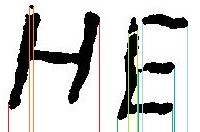
\includegraphics[scale=1]{img/recomposition.jpg}
\caption{Deux groupes de formes sont identifiés (groupe rouge et groupe bleu-vert).}
\end{figure}

Il suffit ensuite de parcourir ce dictionnaire en stockant les formes rencontrées dans une liste séparée et de repérer un saut de x pour passer à un nouveau caractère. La forme complète d'un caractère peut finalement être recomposée.

\subsection{Réanalyse}
A la fin du développement, Guillaume, qui s'occupait de toute la partie segmentation, c'est rendu compte qu'une approche beaucoup plus simple était envisageable: réutiliser le principe de la séparation des lignes qui vérifie sur chaque y de l'image si un point est présent pour cadrer une ligne, mais à la vertical. L'algorithme commencerait par découper horizontalement l'image pour en extraire les lignes, puis verticalement sur chaque ligne pour séparer les caractères et enfin une dernière fois horizontalement sur chaque caractère pour les recadrer (leur hauteur précédente étant celle de la ligne de texte). Les trois étapes serait strictement identiques, seules la dimension et l'image à traiter changeraient.

\begin{figure}[!ht]
\centering
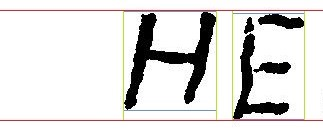
\includegraphics[scale=1]{img/reanalyse.jpg}
\caption{Étapes respectivement en rouge, vert et gris.}
\end{figure}

\subsection{Formatage}
La classification nécessite que l'image à identifier ait une dimension de 28 pixels par 28, mais la représentation du caractère dans les modèles prennent une place spécifique sur la surface disponible: leur hauteur est d'environ 22 pixels. Une simple règle de trois est appliquée pour redimensionner correctement le caractère, qui est ensuite effectué par Pillow. Enfin, si le caractère s'avère plus large que haut, comme dans le cas du W par exemple, les cotés sont enlevés pour rentrer dans les 28 pixels disponible. L'image formatée du caractère qui a alors une taille maximum de 28 fois 22 pixels est placée sur une image en 28 par 28. C'est cette image qui va être passée au classificateur.

\section{Modifications finales de la classification}

\subsection{CharacterClassifierManager et l’automatisation}
Pour simplifier le déroulement de la prédiction et avoir un programme plus ergonomique, nous avons créé la classe CharacterClassfierManager pour que le code ne soit pas un ensemble de fonctions non commentées et d'autres fonctions commentées.

Cette classe initialise le CharacterClassifier avec la liste des labels et check par elle même si une base de donnée est présente. Si elle existe, elle la récupère grâce à pickle.load(). Ou sinon elle entraîne le Classifier puis sauvegarde la base de donnée.

Avec la création du manager, nous avons décelé un autre problème. Nous avons observé que nos matrices de modèle étaient renversées. Ce renversement avait plusieurs origines possibles. Soit une inversion dans la création des PixelMatrix, donc avec une importance minime pour le Classifier puisque tout serait inversé. Soit une inversion lors du chargement des données de la base MNIST ou de la sauvegarde des différents modèles. Après une multitude de tests, nous avons localisé le bug. Le chargement des données n’étaient pas correctement implémenté. Il s'incrémentait en y x au lieu de s’incrémenter en x y.
Voici le résultat après la suppression du renversement:
\begin{figure}[!ht]
\centering
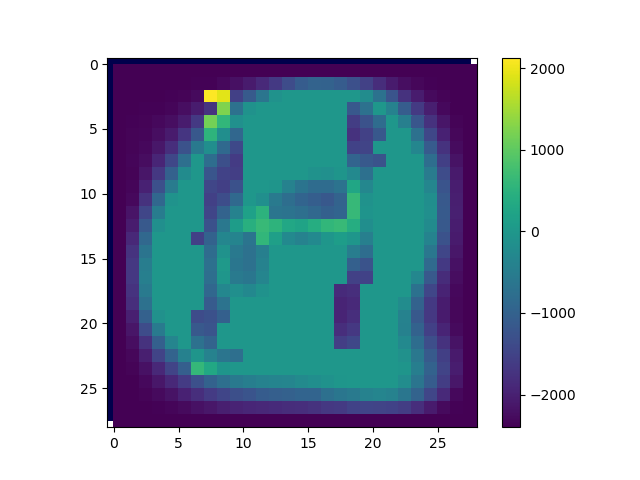
\includegraphics[scale=0.55]{img/pix_corb0.png}
\caption{En bleu-vert, les zones neutres. En jaune, les zones de correspondance entre les 2 matrices. En violet les zones ne correspondant qu'à l'image}
\end{figure}

Cela expliquait en partie les résultats médiocres obtenus lors de la prédiction. Mais malgré cela, on ne pouvait pas dire que le modèle marchait correctement.

\subsection{Utilisation d'une police de caractères comme dataset}
Cependant, nous avons continué à modifier notre modèle pour qu'il soit le plus précis possible. Nous avons donc remplacé le dataset EMNIST avec un dataset basé sur une police de caractères. Les avantages de la police de caractère sont nombreux:
\begin{itemize}
\item Il n'y a pas de variation extravagante dans le modèle. Le modèle a donc une forme plus précise.
\item Le chargement et l'entraînement de la base de donnée est bien plus rapide.
\item L'analyse graphique est plus simple. Il n'y a pas de nuance de points. C'est soit 1 ou -1 dans le modèle.
\end{itemize}

Afin de mieux cerner les problèmes du modèle, nous faisions prédire au CharacterClassifier des images proches du modèle.
Cependant, sur la représentation graphique, il y avait seulement les points de l'image qui étaient communs ou non au modèle.
\begin{figure}[!ht]
\centering
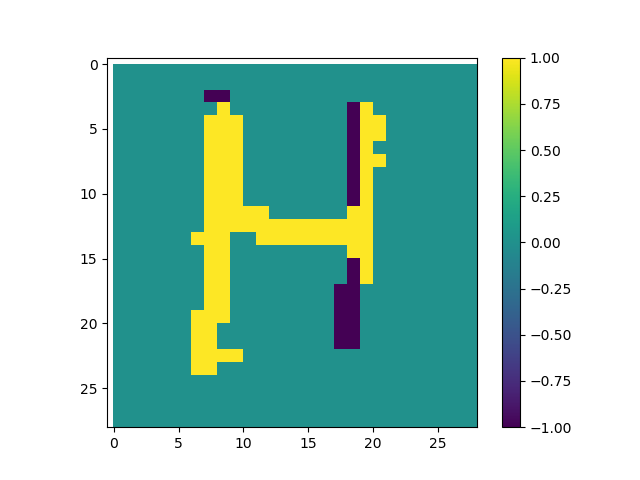
\includegraphics[scale=0.55]{img/pix_cora0.png}
\caption{En jaune, les points de l'image correspondant au modèle. En violet les points de l'image différent du modèle}
\end{figure}

Il fallait donc changer la représentation graphique pour qu'elle corresponde mieux à ce que l'on voulait et ainsi, mieux appréhender les problèmes liés au CharacterClassifier. Nous avons donc rajouter des conditions dans la représentation graphique en comparant à la fois avec la matrice du modèle et la matrice de l’image à prédire.

\begin{figure}[!ht]
\centering
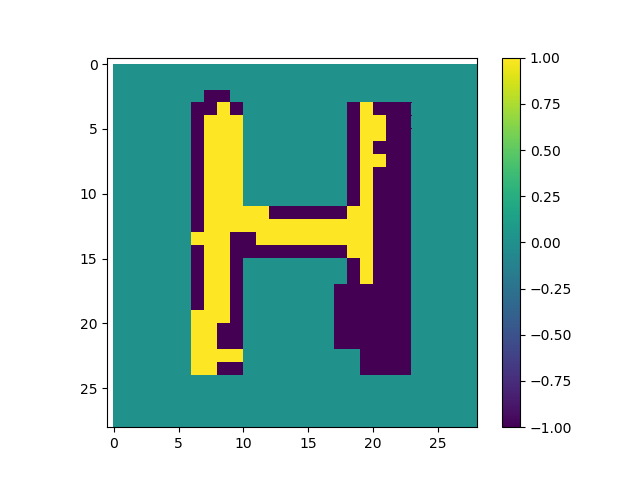
\includegraphics[scale=0.55]{img/pix_cor0.png}
\caption{En jaune, les points de l'image correspondant au modèle. En violet les points de l'image différent du modèle et les points du modèle différents de l'image}
\end{figure}

Graphiquement parlant, cela nous donnait le résultat voulu. Au final, les graphiques de comparaison entre l'image et la bonne matrice n'était pas si différent. Quelque chose modifiait donc nos résultats.

Nous nous sommes rendus comptes qu'en divisant par le score du label, on obtenait des résultats de prédiction faussés car le dénominateur était différent pour chaque score. Deux options s'offrait donc à nous:
\begin{itemize}
\item Enlever la liste des scores des labels
\item Diviser tous les scores de prédictions par tous les scores des labels et baser nos résultats sur l'interprétation des listes de taux obtenus.
\end{itemize}
Nous avons donc décidé de supprimer la liste des scores des labels.

\section{Recombinaison}
Pour le moment, l'OCR a séparé les lignes de texte et pour chacune d'entre elles séparé les caractères avant de les identifier individuellement. Nous nous trouvons à la fin de l'itération de la recherche des caractères de la ligne n. Nous connaissons le code ASCII des caractères mais aussi leur position et leur taille. La largeur moyenne des caractères est calculée et utilisée pour déterminer si la distance entre deux caractères consécutifs correspond à un espace. La chaîne de caractères de la ligne est ainsi reconstituée et ajoutée à la fin du fichier de sortie avant de passer à la ligne n+1.

\section{Architecture du projet}
Ci-dessous le cycle de vie de l'OCR, qui permet d'illustrer les différents appels entre les objets.

\subsection{Cycle de vie de l'OCR}
%----------------------------------------------------------------------------
%-----------------------------------------------------------------------------
%-----------------------------------------------------------------------------
\ifx\du\undefined
  \newlength{\du}
\fi
\setlength{\du}{15\unitlength}
\begin{tikzpicture}
\pgftransformxscale{1.000000}
\pgftransformyscale{-1.000000}
\definecolor{dialinecolor}{rgb}{0.000000, 0.000000, 0.000000}
\pgfsetstrokecolor{dialinecolor}
\definecolor{dialinecolor}{rgb}{1.000000, 1.000000, 1.000000}
\pgfsetfillcolor{dialinecolor}
\pgfsetlinewidth{0.100000\du}
\pgfsetdash{}{0pt}
\pgfsetdash{}{0pt}
\pgfsetmiterjoin
\definecolor{dialinecolor}{rgb}{1.000000, 1.000000, 1.000000}
\pgfsetfillcolor{dialinecolor}
\fill (0.750000\du,0.850000\du)--(0.750000\du,5.250000\du)--(7.650000\du,5.250000\du)--(7.650000\du,0.850000\du)--cycle;
\definecolor{dialinecolor}{rgb}{0.000000, 0.000000, 0.000000}
\pgfsetstrokecolor{dialinecolor}
\draw (0.750000\du,0.850000\du)--(0.750000\du,5.250000\du)--(7.650000\du,5.250000\du)--(7.650000\du,0.850000\du)--cycle;
\pgfsetlinewidth{0.100000\du}
\pgfsetdash{}{0pt}
\pgfsetdash{}{0pt}
\pgfsetmiterjoin
\definecolor{dialinecolor}{rgb}{1.000000, 1.000000, 1.000000}
\pgfsetfillcolor{dialinecolor}
\fill (10.050000\du,0.950000\du)--(10.050000\du,5.250000\du)--(18.050100\du,5.250000\du)--(18.050100\du,0.950000\du)--cycle;
\definecolor{dialinecolor}{rgb}{0.000000, 0.000000, 0.000000}
\pgfsetstrokecolor{dialinecolor}
\draw (10.050000\du,0.950000\du)--(10.050000\du,5.250000\du)--(18.050100\du,5.250000\du)--(18.050100\du,0.950000\du)--cycle;
\pgfsetlinewidth{0.100000\du}
\pgfsetdash{}{0pt}
\pgfsetdash{}{0pt}
\pgfsetmiterjoin
\definecolor{dialinecolor}{rgb}{1.000000, 1.000000, 1.000000}
\pgfsetfillcolor{dialinecolor}
\fill (10.450000\du,9.250000\du)--(10.450000\du,14.050000\du)--(17.950000\du,14.050000\du)--(17.950000\du,9.250000\du)--cycle;
\definecolor{dialinecolor}{rgb}{0.000000, 0.000000, 0.000000}
\pgfsetstrokecolor{dialinecolor}
\draw (10.450000\du,9.250000\du)--(10.450000\du,14.050000\du)--(17.950000\du,14.050000\du)--(17.950000\du,9.250000\du)--cycle;
\pgfsetlinewidth{0.100000\du}
\pgfsetdash{}{0pt}
\pgfsetdash{}{0pt}
\pgfsetmiterjoin
\definecolor{dialinecolor}{rgb}{1.000000, 1.000000, 1.000000}
\pgfsetfillcolor{dialinecolor}
\fill (19.000000\du,9.350000\du)--(19.000000\du,14.750000\du)--(26.800000\du,14.750000\du)--(26.800000\du,9.350000\du)--cycle;
\definecolor{dialinecolor}{rgb}{0.000000, 0.000000, 0.000000}
\pgfsetstrokecolor{dialinecolor}
\draw (19.000000\du,9.350000\du)--(19.000000\du,14.750000\du)--(26.800000\du,14.750000\du)--(26.800000\du,9.350000\du)--cycle;
\pgfsetlinewidth{0.100000\du}
\pgfsetdash{}{0pt}
\pgfsetdash{}{0pt}
\pgfsetmiterjoin
\definecolor{dialinecolor}{rgb}{1.000000, 1.000000, 1.000000}
\pgfsetfillcolor{dialinecolor}
\fill (18.650000\du,17.550000\du)--(18.650000\du,21.100000\du)--(27.450000\du,21.100000\du)--(27.450000\du,17.550000\du)--cycle;
\definecolor{dialinecolor}{rgb}{0.000000, 0.000000, 0.000000}
\pgfsetstrokecolor{dialinecolor}
\draw (18.650000\du,17.550000\du)--(18.650000\du,21.100000\du)--(27.450000\du,21.100000\du)--(27.450000\du,17.550000\du)--cycle;
\pgfsetlinewidth{0.100000\du}
\pgfsetdash{}{0pt}
\pgfsetdash{}{0pt}
\pgfsetmiterjoin
\definecolor{dialinecolor}{rgb}{1.000000, 1.000000, 1.000000}
\pgfsetfillcolor{dialinecolor}
\fill (21.450100\du,25.400000\du)--(21.450100\du,28.650000\du)--(24.350100\du,28.650000\du)--(24.350100\du,25.400000\du)--cycle;
\definecolor{dialinecolor}{rgb}{0.000000, 0.000000, 0.000000}
\pgfsetstrokecolor{dialinecolor}
\draw (21.450100\du,25.400000\du)--(21.450100\du,28.650000\du)--(24.350100\du,28.650000\du)--(24.350100\du,25.400000\du)--cycle;
\pgfsetlinewidth{0.100000\du}
\pgfsetdash{}{0pt}
\pgfsetdash{}{0pt}
\pgfsetmiterjoin
\definecolor{dialinecolor}{rgb}{1.000000, 1.000000, 1.000000}
\pgfsetfillcolor{dialinecolor}
\fill (3.250000\du,20.400000\du)--(3.250000\du,25.100000\du)--(12.550000\du,25.100000\du)--(12.550000\du,20.400000\du)--cycle;
\definecolor{dialinecolor}{rgb}{0.000000, 0.000000, 0.000000}
\pgfsetstrokecolor{dialinecolor}
\draw (3.250000\du,20.400000\du)--(3.250000\du,25.100000\du)--(12.550000\du,25.100000\du)--(12.550000\du,20.400000\du)--cycle;
\pgfsetlinewidth{0.100000\du}
\pgfsetdash{}{0pt}
\pgfsetdash{}{0pt}
\pgfsetmiterjoin
\definecolor{dialinecolor}{rgb}{1.000000, 1.000000, 1.000000}
\pgfsetfillcolor{dialinecolor}
\fill (20.150000\du,30.750000\du)--(20.150000\du,34.450000\du)--(25.750000\du,34.450000\du)--(25.750000\du,30.750000\du)--cycle;
\definecolor{dialinecolor}{rgb}{0.000000, 0.000000, 0.000000}
\pgfsetstrokecolor{dialinecolor}
\draw (20.150000\du,30.750000\du)--(20.150000\du,34.450000\du)--(25.750000\du,34.450000\du)--(25.750000\du,30.750000\du)--cycle;
\pgfsetlinewidth{0.100000\du}
\pgfsetdash{}{0pt}
\pgfsetdash{}{0pt}
\pgfsetbuttcap
{
\definecolor{dialinecolor}{rgb}{0.000000, 0.000000, 0.000000}
\pgfsetfillcolor{dialinecolor}
% was here!!!
\pgfsetarrowsend{stealth}
\definecolor{dialinecolor}{rgb}{0.000000, 0.000000, 0.000000}
\pgfsetstrokecolor{dialinecolor}
\draw (7.699581\du,3.067764\du)--(9.999770\du,3.079440\du);
}
\pgfsetlinewidth{0.100000\du}
\pgfsetdash{}{0pt}
\pgfsetdash{}{0pt}
\pgfsetbuttcap
{
\definecolor{dialinecolor}{rgb}{0.000000, 0.000000, 0.000000}
\pgfsetfillcolor{dialinecolor}
% was here!!!
\pgfsetarrowsend{stealth}
\definecolor{dialinecolor}{rgb}{0.000000, 0.000000, 0.000000}
\pgfsetstrokecolor{dialinecolor}
\draw (14.088599\du,5.298035\du)--(14.157058\du,9.201477\du);
}
\pgfsetlinewidth{0.100000\du}
\pgfsetdash{}{0pt}
\pgfsetdash{}{0pt}
\pgfsetbuttcap
{
\definecolor{dialinecolor}{rgb}{0.000000, 0.000000, 0.000000}
\pgfsetfillcolor{dialinecolor}
% was here!!!
\pgfsetarrowsend{stealth}
\definecolor{dialinecolor}{rgb}{0.000000, 0.000000, 0.000000}
\pgfsetstrokecolor{dialinecolor}
\draw (18.000409\du,11.824731\du)--(18.953564\du,11.868555\du);
}
\pgfsetlinewidth{0.100000\du}
\pgfsetdash{}{0pt}
\pgfsetdash{}{0pt}
\pgfsetbuttcap
{
\definecolor{dialinecolor}{rgb}{0.000000, 0.000000, 0.000000}
\pgfsetfillcolor{dialinecolor}
% was here!!!
\pgfsetarrowsend{stealth}
\definecolor{dialinecolor}{rgb}{0.000000, 0.000000, 0.000000}
\pgfsetstrokecolor{dialinecolor}
\draw (22.956699\du,14.799883\du)--(23.012427\du,17.502698\du);
}
\pgfsetlinewidth{0.100000\du}
\pgfsetdash{}{0pt}
\pgfsetdash{}{0pt}
\pgfsetbuttcap
{
\definecolor{dialinecolor}{rgb}{0.000000, 0.000000, 0.000000}
\pgfsetfillcolor{dialinecolor}
% was here!!!
\pgfsetarrowsend{stealth}
\definecolor{dialinecolor}{rgb}{0.000000, 0.000000, 0.000000}
\pgfsetstrokecolor{dialinecolor}
\draw (23.014483\du,21.149426\du)--(22.932717\du,25.349554\du);
}
\pgfsetlinewidth{0.100000\du}
\pgfsetdash{}{0pt}
\pgfsetdash{}{0pt}
\pgfsetbuttcap
{
\definecolor{dialinecolor}{rgb}{0.000000, 0.000000, 0.000000}
\pgfsetfillcolor{dialinecolor}
% was here!!!
\pgfsetarrowsstart{stealth}
\pgfsetarrowsend{stealth}
\definecolor{dialinecolor}{rgb}{0.000000, 0.000000, 0.000000}
\pgfsetstrokecolor{dialinecolor}
\draw (22.499738\du,22.718146\du)--(12.600093\du,22.739745\du);
}
\pgfsetlinewidth{0.100000\du}
\pgfsetdash{}{0pt}
\pgfsetdash{}{0pt}
\pgfsetbuttcap
{
\definecolor{dialinecolor}{rgb}{0.000000, 0.000000, 0.000000}
\pgfsetfillcolor{dialinecolor}
% was here!!!
\pgfsetarrowsend{stealth}
\definecolor{dialinecolor}{rgb}{0.000000, 0.000000, 0.000000}
\pgfsetstrokecolor{dialinecolor}
\draw (22.915091\du,28.699814\du)--(22.933017\du,30.702649\du);
}
% setfont left to latex
\definecolor{dialinecolor}{rgb}{0.000000, 0.000000, 0.000000}
\pgfsetstrokecolor{dialinecolor}
\node[anchor=west] at (2.100000\du,2.950000\du){utils.graphics};
% setfont left to latex
\definecolor{dialinecolor}{rgb}{0.000000, 0.000000, 0.000000}
\pgfsetstrokecolor{dialinecolor}
\node[anchor=west] at (2.100000\du,3.750000\du){RawImage};
% setfont left to latex
\definecolor{dialinecolor}{rgb}{0.000000, 0.000000, 0.000000}
\pgfsetstrokecolor{dialinecolor}
\node[anchor=west] at (4.700000\du,22.450000\du){analysis.recognition};
% setfont left to latex
\definecolor{dialinecolor}{rgb}{0.000000, 0.000000, 0.000000}
\pgfsetstrokecolor{dialinecolor}
\node[anchor=west] at (4.700000\du,23.250000\du){CharacterClassifier};
% setfont left to latex
\definecolor{dialinecolor}{rgb}{0.000000, 0.000000, 0.000000}
\pgfsetstrokecolor{dialinecolor}
\node[anchor=west] at (10.550000\du,3.150000\du){analysis.graphics.text};
% setfont left to latex
\definecolor{dialinecolor}{rgb}{0.000000, 0.000000, 0.000000}
\pgfsetstrokecolor{dialinecolor}
\node[anchor=west] at (10.550000\du,3.950000\du){TextLineDiscovery};
\pgfsetlinewidth{0.100000\du}
\pgfsetdash{}{0pt}
\pgfsetdash{}{0pt}
\pgfsetbuttcap
{
\definecolor{dialinecolor}{rgb}{0.000000, 0.000000, 0.000000}
\pgfsetfillcolor{dialinecolor}
% was here!!!
\pgfsetarrowsend{stealth}
\definecolor{dialinecolor}{rgb}{0.000000, 0.000000, 0.000000}
\pgfsetstrokecolor{dialinecolor}
\pgfpathmoveto{\pgfpoint{13.950115\du}{6.799992\du}}
\pgfpatharc{245}{-86}{0.508125\du and 0.508125\du}
\pgfusepath{stroke}
}
% setfont left to latex
\definecolor{dialinecolor}{rgb}{0.000000, 0.000000, 0.000000}
\pgfsetstrokecolor{dialinecolor}
\node[anchor=west] at (15.850100\du,7.050000\du){For every line};
% setfont left to latex
\definecolor{dialinecolor}{rgb}{0.000000, 0.000000, 0.000000}
\pgfsetstrokecolor{dialinecolor}
\node[anchor=west] at (12.500000\du,11.450000\du){utils.graphics};
% setfont left to latex
\definecolor{dialinecolor}{rgb}{0.000000, 0.000000, 0.000000}
\pgfsetstrokecolor{dialinecolor}
\node[anchor=west] at (12.500000\du,12.250000\du){TextLine};
% setfont left to latex
\definecolor{dialinecolor}{rgb}{0.000000, 0.000000, 0.000000}
\pgfsetstrokecolor{dialinecolor}
\node[anchor=west] at (19.650000\du,11.700000\du){analysis.graphics.text};
% setfont left to latex
\definecolor{dialinecolor}{rgb}{0.000000, 0.000000, 0.000000}
\pgfsetstrokecolor{dialinecolor}
\node[anchor=west] at (19.650000\du,12.500000\du){CharacterDiscovery};
\pgfsetlinewidth{0.100000\du}
\pgfsetdash{}{0pt}
\pgfsetdash{}{0pt}
\pgfsetbuttcap
{
\definecolor{dialinecolor}{rgb}{0.000000, 0.000000, 0.000000}
\pgfsetfillcolor{dialinecolor}
% was here!!!
\pgfsetarrowsend{stealth}
\definecolor{dialinecolor}{rgb}{0.000000, 0.000000, 0.000000}
\pgfsetstrokecolor{dialinecolor}
\pgfpathmoveto{\pgfpoint{22.950115\du}{15.399997\du}}
\pgfpatharc{259}{-78}{0.505000\du and 0.505000\du}
\pgfusepath{stroke}
}
% setfont left to latex
\definecolor{dialinecolor}{rgb}{0.000000, 0.000000, 0.000000}
\pgfsetstrokecolor{dialinecolor}
\node[anchor=west] at (20.950000\du,32.700000\du){output.txt};
% setfont left to latex
\definecolor{dialinecolor}{rgb}{0.000000, 0.000000, 0.000000}
\pgfsetstrokecolor{dialinecolor}
\node[anchor=west] at (15.450100\du,16.250000\du){For every Character};
% setfont left to latex
\definecolor{dialinecolor}{rgb}{0.000000, 0.000000, 0.000000}
\pgfsetstrokecolor{dialinecolor}
\node[anchor=west] at (20.650000\du,19.575000\du){utils.graphics.text};
% setfont left to latex
\definecolor{dialinecolor}{rgb}{0.000000, 0.000000, 0.000000}
\pgfsetstrokecolor{dialinecolor}
\node[anchor=west] at (20.650000\du,20.375000\du){Character};
% setfont left to latex
\definecolor{dialinecolor}{rgb}{0.000000, 0.000000, 0.000000}
\pgfsetstrokecolor{dialinecolor}
\node[anchor=west] at (15.750100\du,23.600000\du){predict};
% setfont left to latex
\definecolor{dialinecolor}{rgb}{0.000000, 0.000000, 0.000000}
\pgfsetstrokecolor{dialinecolor}
\node[anchor=west] at (22.300100\du,27.325000\du){"A"};
\end{tikzpicture}
%-----------------------------------------------------------------------------


\pagebreak
\subsection{Modules}
Notre application a été scindée en de nombreux modules pour que le code soit facilement réutilisable.

\dirtree{%
.1 .
.2 analysis \ldots{} \begin{minipage}[t]{10cm}
Module d'analyses{.}
\end{minipage}.
.3 graphics \ldots{} \begin{minipage}[t]{10cm}
Module d'analyses graphiques{.} Contient la classe ShapeDiscovery qui implémente l'algorithme d'extraction de formes{.}
\end{minipage}.
.4 text \ldots{} \begin{minipage}[t]{10cm}
Module d'analyses d'images de textes{.} Contient les classes TextLineDiscovery et CharacterDiscovery qui implémentent respectivement l'algorithme de recherche de lignes de texte et l'algorithme de recherche de caractères{.}
\end{minipage}.
.3 recognition \ldots{} \begin{minipage}[t]{10cm}
Module de reconnaissance d'images{.} Contient la classe MatricePoids qui représente un modèle, la classe CharacterFormatter qui formate les caractères extraits pour les reconnaître, la classe CharacterClassifier qui implémente l'algorithme de classification et la classe CharacterClassifier qui automatise les opérations d’entraînement et de chargement du classificateur{.}
\end{minipage}.
.2 dataset \ldots{} \begin{minipage}[t]{10cm}
Module de lecture du dataset{.}
\end{minipage}.
.2 utils \ldots{} \begin{minipage}[t]{10cm}
Module d'objets de base{.} Contient les classes Point et Matrix utilisées à travers toute l'application{.}
\end{minipage}.
.3 graphics \ldots{} \begin{minipage}[t]{10cm}
Module d'objets graphiques de base{.} Contient les classes PixelMatrix, RawImage et Shape{.}
\end{minipage}.
.4 text \ldots{} \begin{minipage}[t]{10cm}
Module d'objets graphiques textuels de base{.} Contient les classes Character et TextLine{.}
\end{minipage}.
}

\pagebreak
\part{Conclusion}
\section{Bilan}
En prenant l'image "HELLO WORLD", le résultat retourné est "HJDKQ UQKKD" pour le modèle avec EMNIST et "HLLLD WOBLB" avec le modèle police de caractères.

Le taux de succès de notre OCR est bas, principalement à cause de la faible précision du modèle avec EMNIST et la rigidité de celui avec la police de caractère, ce dernier ne faisant finalement plus appel à l'apprentissage machine puisqu'il compare l'image à identifier avec les caractères présents dans la police. Nous avons dû ajouter des règles d'écriture importantes pour faire en sorte que l'OCR fonctionne correctement. Sans surprise, pour maximiser la reconnaissance avec le deuxième modèle, il faut que les caractères à identifier soient quasi similaires à leur modèle correspondant.

\section{Possibilités d'améliorations}
Comme nous l'avons montrer plus haut, notre OCR n'est pas parfait et il existe différentes façons de l'améliorer
\begin{itemize}
\item Pour augmenter la précision, nous pouvons modifier l'algorithme pixel pour le transformer en algorithme vectoriel. En effet, le modèle pixel par pixel est trop dépendant des variations et du bruit. Une reconnaissance de forme serait plus précise pour des lettres. Ou pourquoi pas combiner les deux.

\item Ou encore, nous pouvons changer la taille des matrices nous servant de modèle. Au lieu de la dimension 28*28 qui nous a été imposé par EMNIST, nous pouvons prendre une dimension en 100*100. Cela créerait plus de détails sur chaque image et le poids relatif de chaque pixel serait plus petit, rendant par conséquent l'algorithme pixel par pixel plus puissant, plus précis. Mais la  vitesse d'entraînement et la rapidité de prédiction en seraient affectées.
\end{itemize}
\end{document}
